\maketitle
\tableofcontents
\newpage

\section{Zielsetzung}
In diesem Versuch geht es um die Untersuchung der Wärmeleitung von Aluminium, Edelstahl und Messing.
\section{Theorie}
Wärmeleitung ist eine von drei Methoden, um Wärme entlang eines Temperaturgefälles zu transportieren,
welches durch eine Störung des Temperaturgleichgewichts ensteht. Neben Konvektion und Wärmestrahlung
erfolgt die Wärmeleitung durch Phononen und frei bewegliche Elektronen. Durch einen Stab der Länge L und der
Querschnittsfläche A, der aus einem Material mit Dichte $\textit{\rho}$ und spezifische Wärme $\textit{c}$ besteht,
fließt in der Zeit $\textit{dt}$ bezüglich der Querschnittsfläche die Wärmemenge
\begin{equation}
  \symup dQ = - \kappa \, A \, \frac{\partial T}{\partial x} \, \symup dt .
  \label{eqn:1}
\end{equation}
Dabei ist $\kappa$ die materialabhängige Wärmeleitfähigkeit. Mit Hilfe der Wärmestromdichte
$j_{\omega}$ und Wärmeleitungsgleichung lässt sich die Temperaturwellengleichung schreiben als
\begin{equation}
  T(x, t) = T_{max} \ e^{\sqrt{\frac{\omega \rho c}{2 \kappa}} \, x} \,
  cos \left(\omega t - \sqrt{\frac{\omega \rho c}{2 \kappa}} \, x \right)
  \label{eqn:2}
\end{equation}
für einen mit Periode T abwechselnd erwärmten und abgekühlten sehr langen Stab.
Die Phasengesschwindigkeit der Welle lautet
\begin{equation}
    v = \frac{\omega}{k} = \frac{\omega}{\sqrt{\frac{\omega \rho c}{2 \kappa}}}
    = \sqrt{\frac{2 \kappa \omega}{\rho c}}
    \label{eqn:3}
\end{equation}
zur Bestimmung der Dämpfung nutzt man das Amplitudenverhältnis aus $A_{nah}$ und $A_{fern}$
an zwei Messstellen $x_{nah}$ und $x_{fern}$. Für die Wärmeleitfähigkeit erhält man also
\begin{equation}
  \kappa = \frac{\rho c (\Delta x)^2}{2 \, \Delta t \, ln (A_{nah}/{A_{fern})}}
  \label{eqn:4}
\end{equation}
mit $\Delta x$ als Abstand und $\Delta t$ als Phasendifferenz der Temperaturwelle
zwischen den beiden Messstellen.
\section{Durchführung}
\subsection{Versuchsaufbau}
Auf der Grundplatte sind vier rechteckige Probestäbe aus Aluminium, zweimal Messing
und Edelstahl. Ein Peltierelement erhitzt bzw. kühlt die Probestäbe gleichzeitig.
Mit einem Schalter lässt sich zwischen diesen beiden Betriebsarten umschalten.
Die Eingangsspannungen sind 5 $\textit{V}$ für die statische bzw. 8 $\textit{V}$
für die dynamische Methode \footnote{Siehe \ref{sec:1}}. Die Temperaturen werden
an zwei Stellen eines Stabes abgegriffen und an einen Datenlogger (Xplorer GLX)
weitergeleitet.
\begin{figure}
  \centering
  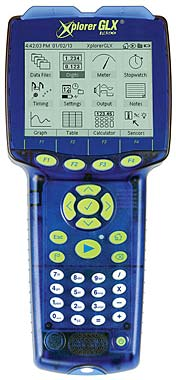
\includegraphics[scale=0.5]{xplorer_glx.jpg}
  \caption{Darstellung eines Datenloggers Typ Xplorer GLX.}
  \label{fig:1}
\end{figure}
\begin{figure}
  \centering
  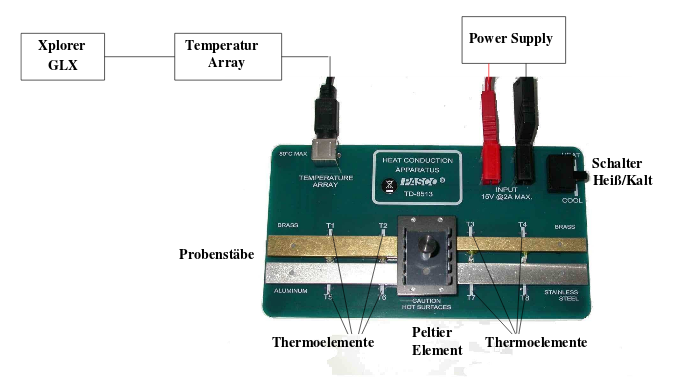
\includegraphics[scale=0.5]{versuchsaufbau.png}
  \caption{Versuchsuafbau.}
  \label{fig:2}
\end{figure}
\subsection{Versuchsdurchführung}
\label{sec:1}
Zu Beginn des Versuchs und nach jedem Abkühlvorgang isolieren wir die Metallstäbe,
um den Wärmeaustausch mit der Umgebungs so gering wie möglich zu halten. Es werden
zwei verschiedene Messmethoden angewandt:
\begin{itemize}
  \item Statistische Methode:
    Über den zeitliche Temperaturverlauf wird die Wärmeleitfähigkeit bestimmt.
    Zu diesem Zweck werden an zwei Messstellen eines jeden Metallstabs die Temperatur
    als Funktion der Zeit dargestellt.
  \item Dynamische Methode
\end{itemize}
\section{Auswertung}
\subsection{Statische Methode}
Alle Temperaturverläufe haben einen exponentiellen Verlauf. 

Die Betrachtung der Temperaturverläufe an den entfernt liegenden Termoelementen zeigt, dass Aluminium die höchste
Wärmeleitfähigkeit besitzt. Auf Aluminium folgen Messing und schließlich Edelstahl, welches die geringste Wärmeleitfähigkeit der
betrachteten Metalle aufweist. Aus dem Verlauf der Temperaturkurven der beiden Messingstäbe folgt, dass aus einem höherer Querschnitt
eine höhere Wärmeleitung folgt.


\section{Diskussion}
\newpage
\nocite{*}
\printbibliography
